\documentclass{standalone}
\usepackage{ tikz }
\usetikzlibrary{shapes}
\usetikzlibrary{plotmarks}
\usepackage{ xparse }
\usepackage{../../../macros}

\begin{document}
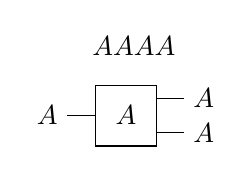
\begin{tikzpicture}[yscale=-1,x=1em,y=1.25em]
        
    \node at (1.4,-2) {$\morph{\ccopy{A}}{A}{A \tensor A}$};

    \node [anchor=east] at (-1,0) {$A$};
    \draw (-1,0) -- (0,0);
    \node[draw, minimum height = 2.2em, minimum width = 2.2em, anchor = west] at (0,0){$\ccopy{A}$};
    \draw (2.2,-0.5) -- (3.2,-0.5);
    \draw (2.2,0.5) -- (3.2,0.5);
    \node [anchor=west] at (3.2,-0.5) {$A$};
    \node [anchor=west] at (3.2,0.5) {$A$};

\end{tikzpicture}
\end{document}